\documentclass[12pt]{article}
\usepackage[T1]{fontenc}
\usepackage[utf8]{inputenc}
\usepackage[margin=1.2in]{geometry}
\usepackage{graphicx}
\usepackage{mathtools}
\usepackage{indentfirst}
\usepackage{float}
\usepackage{listings}
\usepackage{tabularx}
\usepackage{array}
\usepackage{wrapfig}
\usepackage{multirow}
\usepackage{graphicx} %Loading the package
\usepackage{verbatim}
\graphicspath{{../figs/}} %Setting the graphicspath

\usepackage[dvipsnames]{xcolor}

\usepackage{fancyvrb}

% redefine \VerbatimInput
\RecustomVerbatimCommand{\VerbatimInput}{VerbatimInput}%
{fontsize=\footnotesize,
 %
 frame=lines,  % top and bottom rule only
 framesep=2em, % separation between frame and text
 rulecolor=\color{Gray},
 %
 label=\fbox{\color{Black}Params},
 labelposition=topline,
 %
 commandchars=\|\(\), % escape character and argument delimiters for
                      % commands within the verbatim
 commentchar=*        % comment character
}

\usepackage{pdfpages} 

\title{AEM 4305 - SADC \\ Semester Project Part 2: \\ MayFly Mission }
\author{By: Garrett Ailts \\ }
\date{Mar 7 2020}

\begin{document}
\maketitle
\thispagestyle{empty}
\newpage

\section{Orbital Dynamics and Equations of Motion}
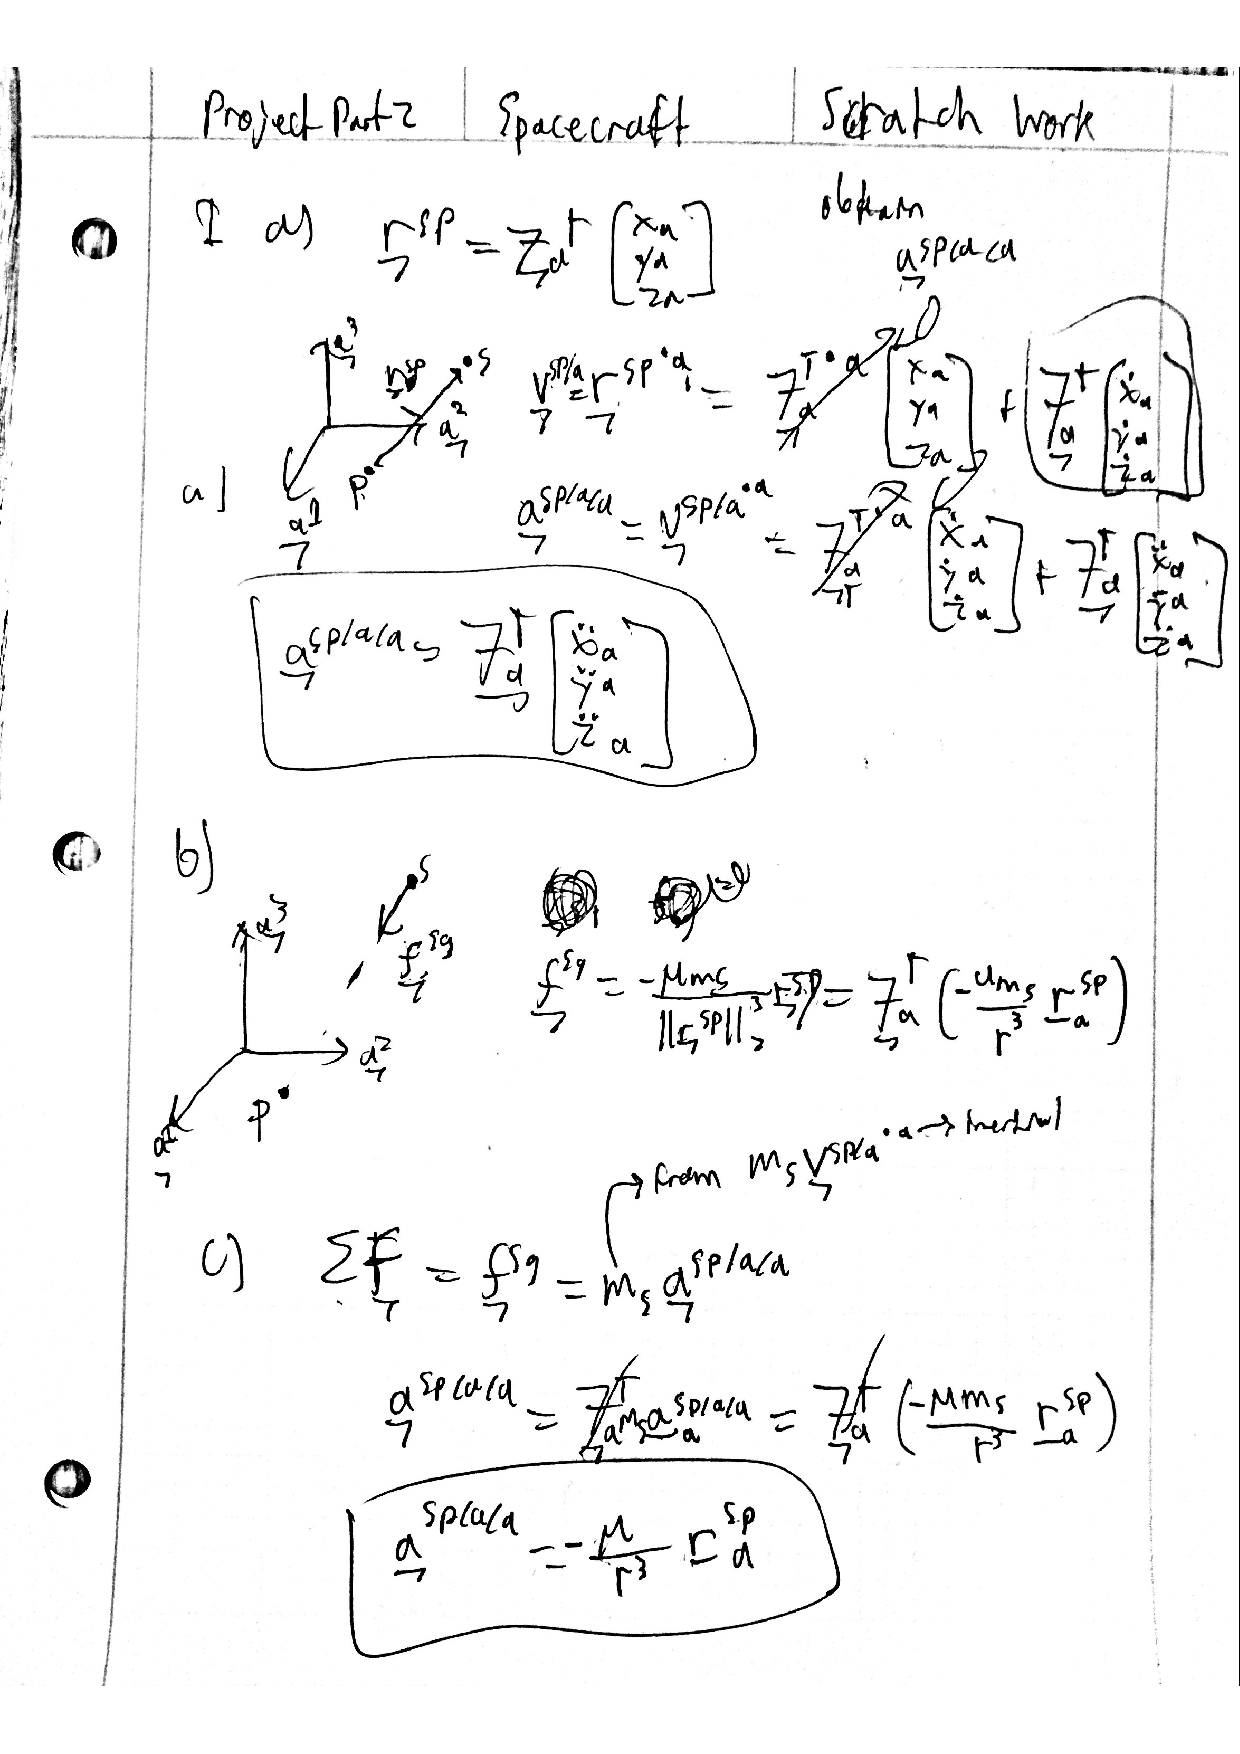
\includepdf[pages=-]{Semester_Project/docs/pdf/Spacecraft_Project_P2}


%\VerbatimInput{Semester_Project/params/scParams.txt}
\newpage

\section{Numerical Simulation of Orbital Dynamics}
First, the spacecraft is simulated without the J2 Perturbation. The following outputs show the spacecrafts position and velocity in the ECI frame, as well as the total energy and energy change.

\begin{figure}[H]
\centering
    \includegraphics[width=0.7\textwidth]{Semester_Project/figs/PMO_J2off/sc_position.png}
    \caption{Cartesian position of spacecraft in km}
\end{figure}
\begin{figure}[H]
\centering
    \includegraphics[width=0.7\textwidth]{Semester_Project/figs/PMO_J2off/sc_velocity.png}
    \caption{Cartesian velocity of spacecraft in km/s}
\end{figure}
\begin{figure}[H]
\centering
    \includegraphics[width=0.7\textwidth]{Semester_Project/figs/PMO_J2off/EarthPlot.png}
    \caption{Spacecraft orbit around Earth in the ECI frame}
\end{figure}
\begin{figure}[H]
\centering
    \includegraphics[width=0.7\textwidth]{Semester_Project/figs/PMO_J2off/sc_energy.png}
    \caption{Energy and energy normalized by the starting energy of spacecraft}
\end{figure}

\newpage
Now the spacecraft is simulated with the inclusion of the J2 perturbation.

% redefine \VerbatimInput
\RecustomVerbatimCommand{\VerbatimInput}{VerbatimInput}%
{fontsize=\footnotesize,
 %
 frame=lines,  % top and bottom rule only
 framesep=2em, % separation between frame and text
 rulecolor=\color{Gray},
 %
 label=\fbox{\color{Black}earthParams.txt},
 labelposition=topline,
 %
 commandchars=\|\(\), % escape character and argument delimiters for
                      % commands within the verbatim
 commentchar=*        % comment character
}
\VerbatimInput{Semester_Project/params/earthParams.txt}

\begin{figure}[H]
\centering
    \includegraphics[width=0.7\textwidth]{Semester_Project/figs/PMO_J2on/sc_position.png}
    \caption{Cartesian position of spacecraft in km}
\end{figure}
\begin{figure}[H]
\centering
    \includegraphics[width=0.7\textwidth]{Semester_Project/figs/PMO_J2on/sc_velocity.png}
    \caption{Cartesian velocity of spacecraft in km/s}
\end{figure}
\begin{figure}[H]
\centering
    \includegraphics[width=0.7\textwidth]{Semester_Project/figs/PMO_J2on/EarthPlot.png}
    \caption{Spacecraft orbit around Earth in the ECI frame}
\end{figure}
\begin{figure}[H]
\centering
    \includegraphics[width=0.7\textwidth]{Semester_Project/figs/PMO_J2on/sc_energy.png}
    \caption{Energy and energy normalized by the starting energy of spacecraft}
\end{figure}

Below are inclusions of my versions of the following MATLAB functions: constants\_struct.m, main compile.m, ODEs.m, and
post\_processing.m. Constants struct is split into a parameter loader function and a simulation driver file that loads all the correct parameters and adds the desired directories to path.

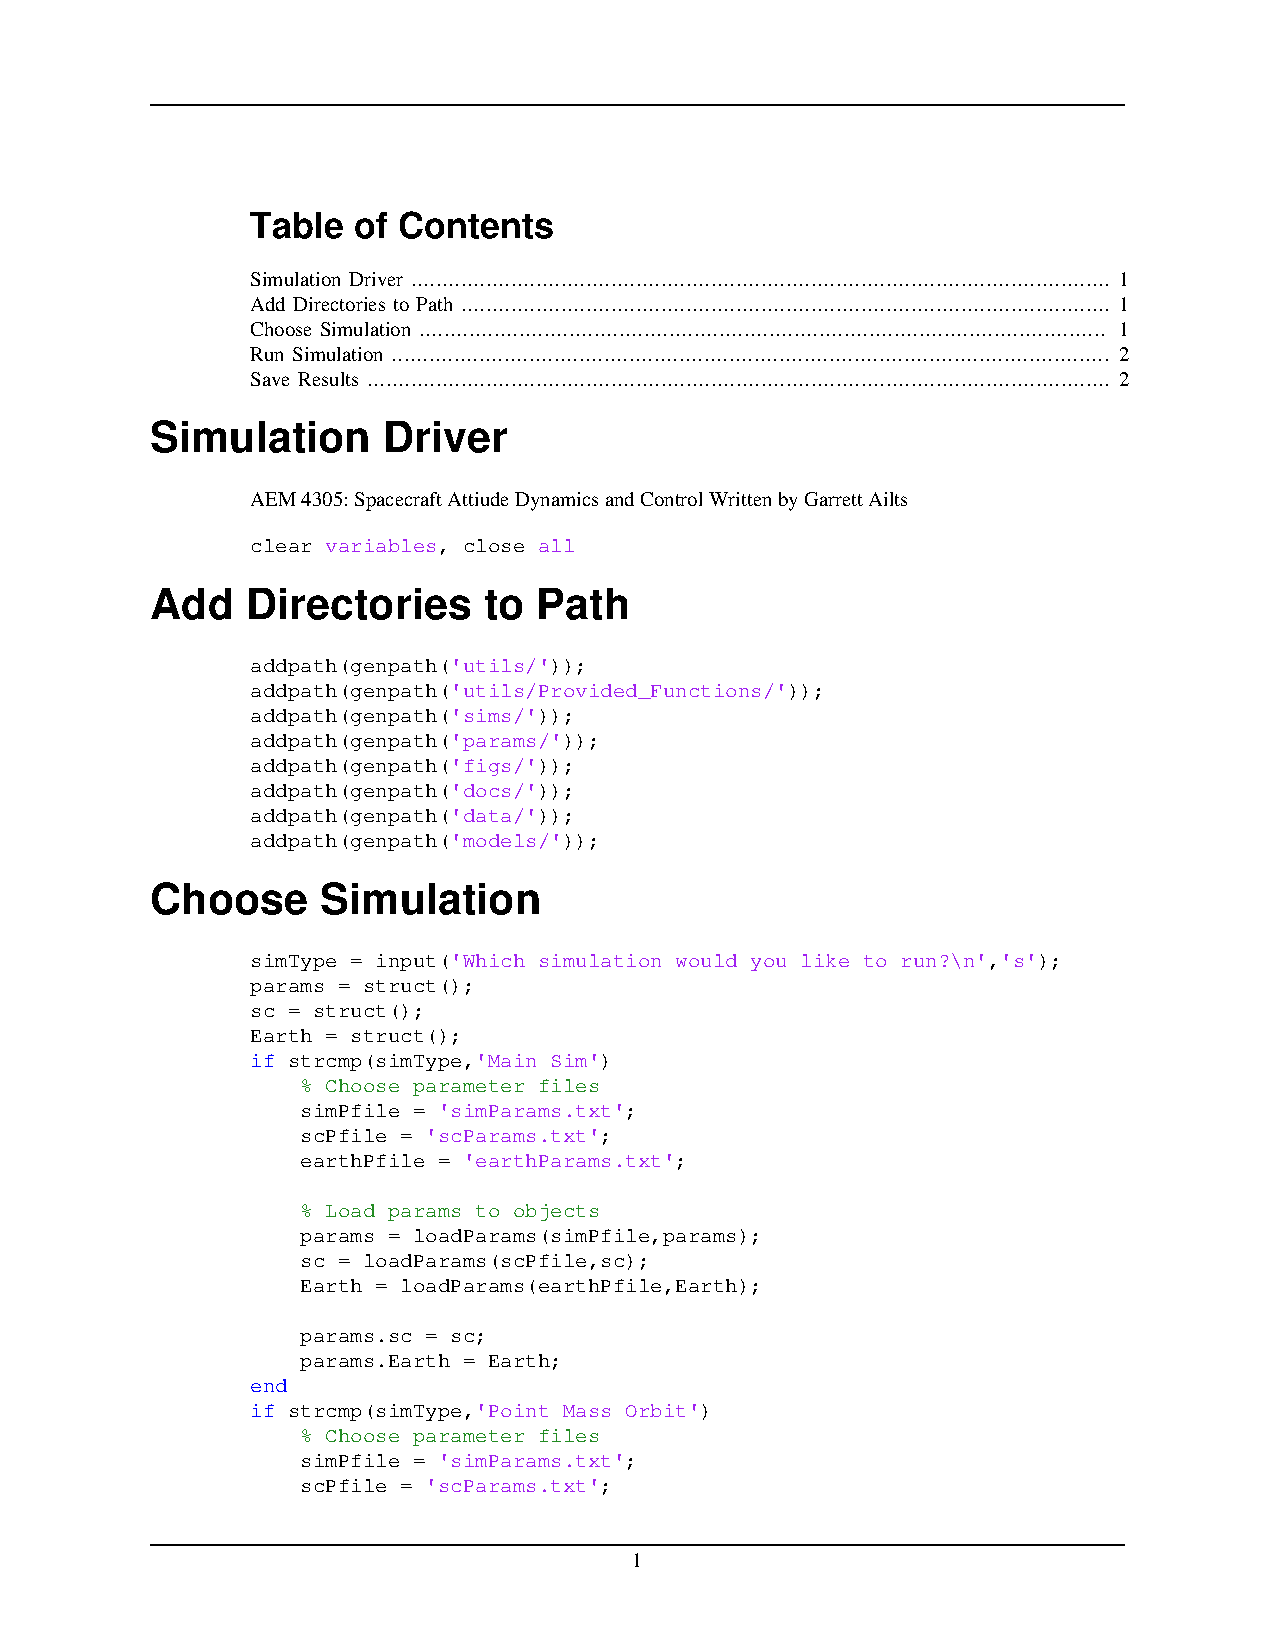
\includepdf[pages=-]{Semester_Project/docs/pdf/simDriver.pdf}
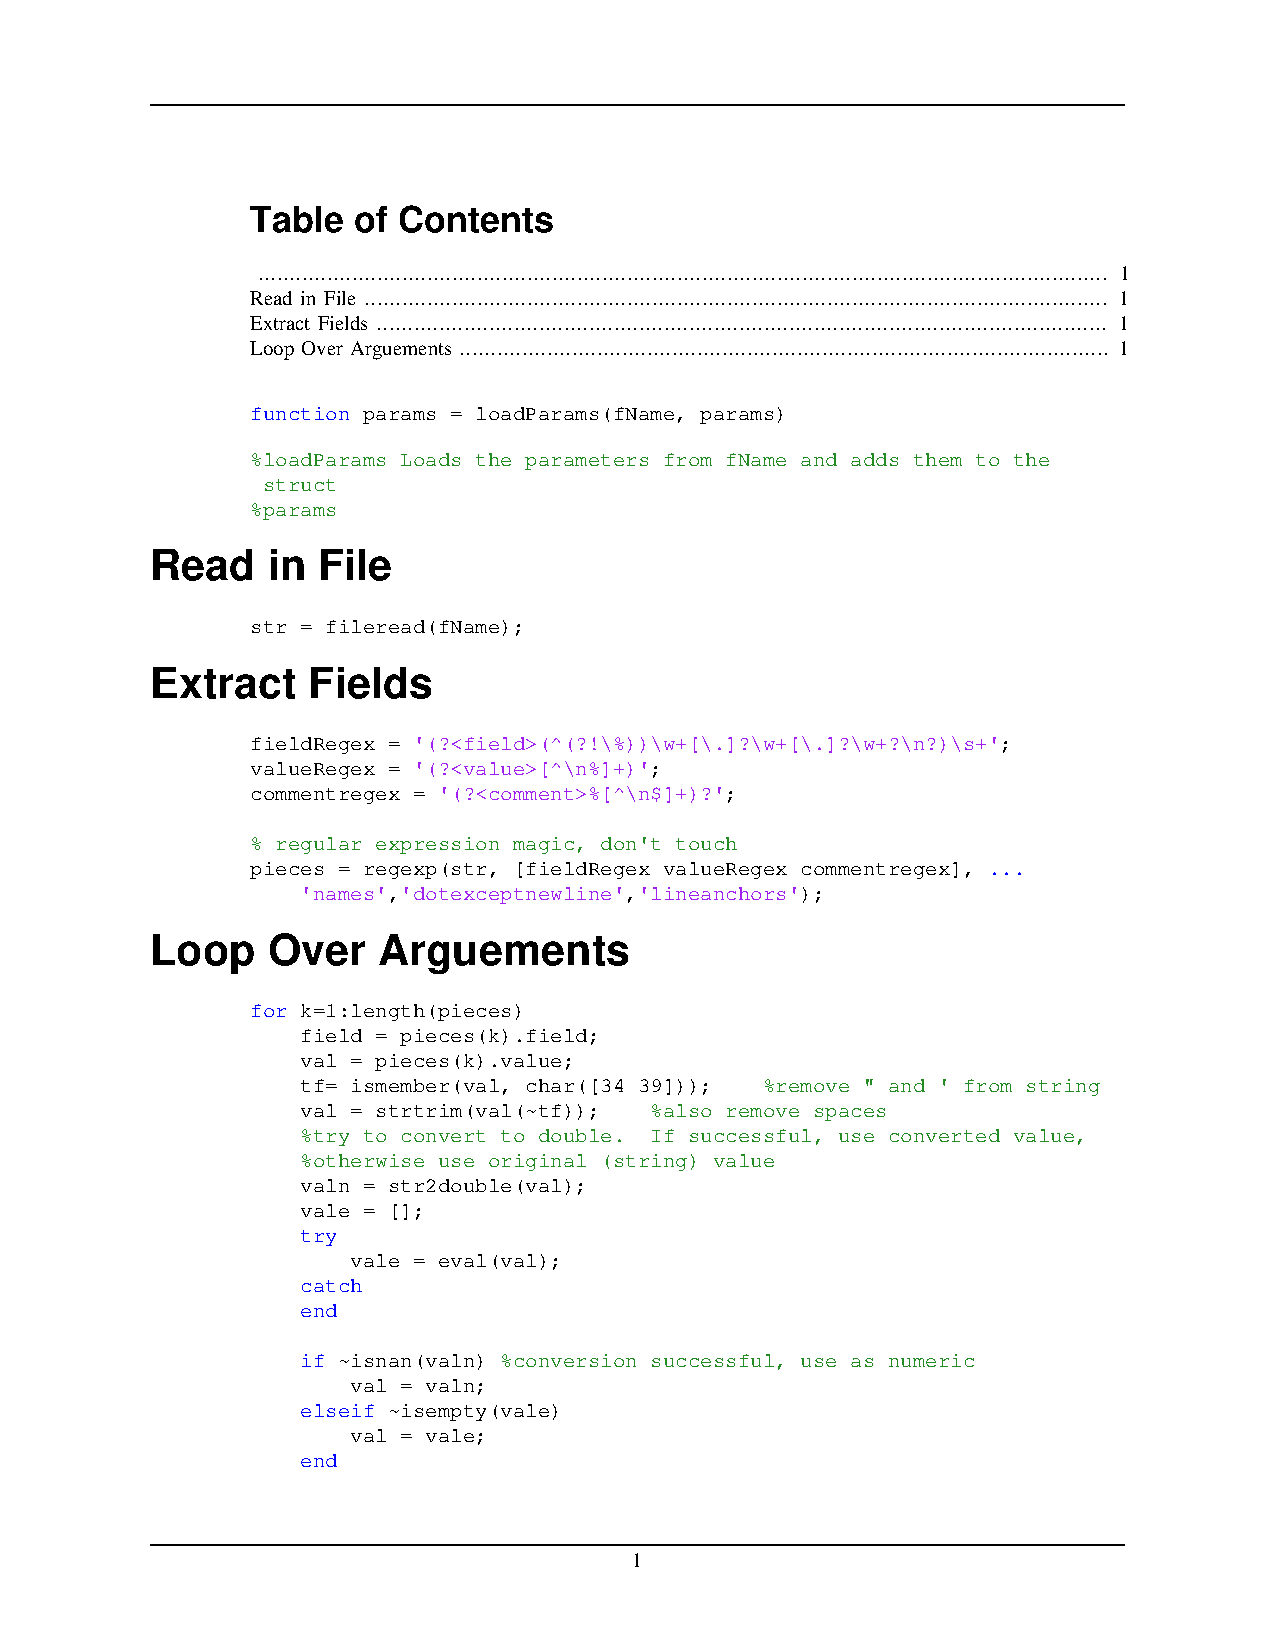
\includepdf[pages=-]{Semester_Project/docs/pdf/loadParams.pdf}
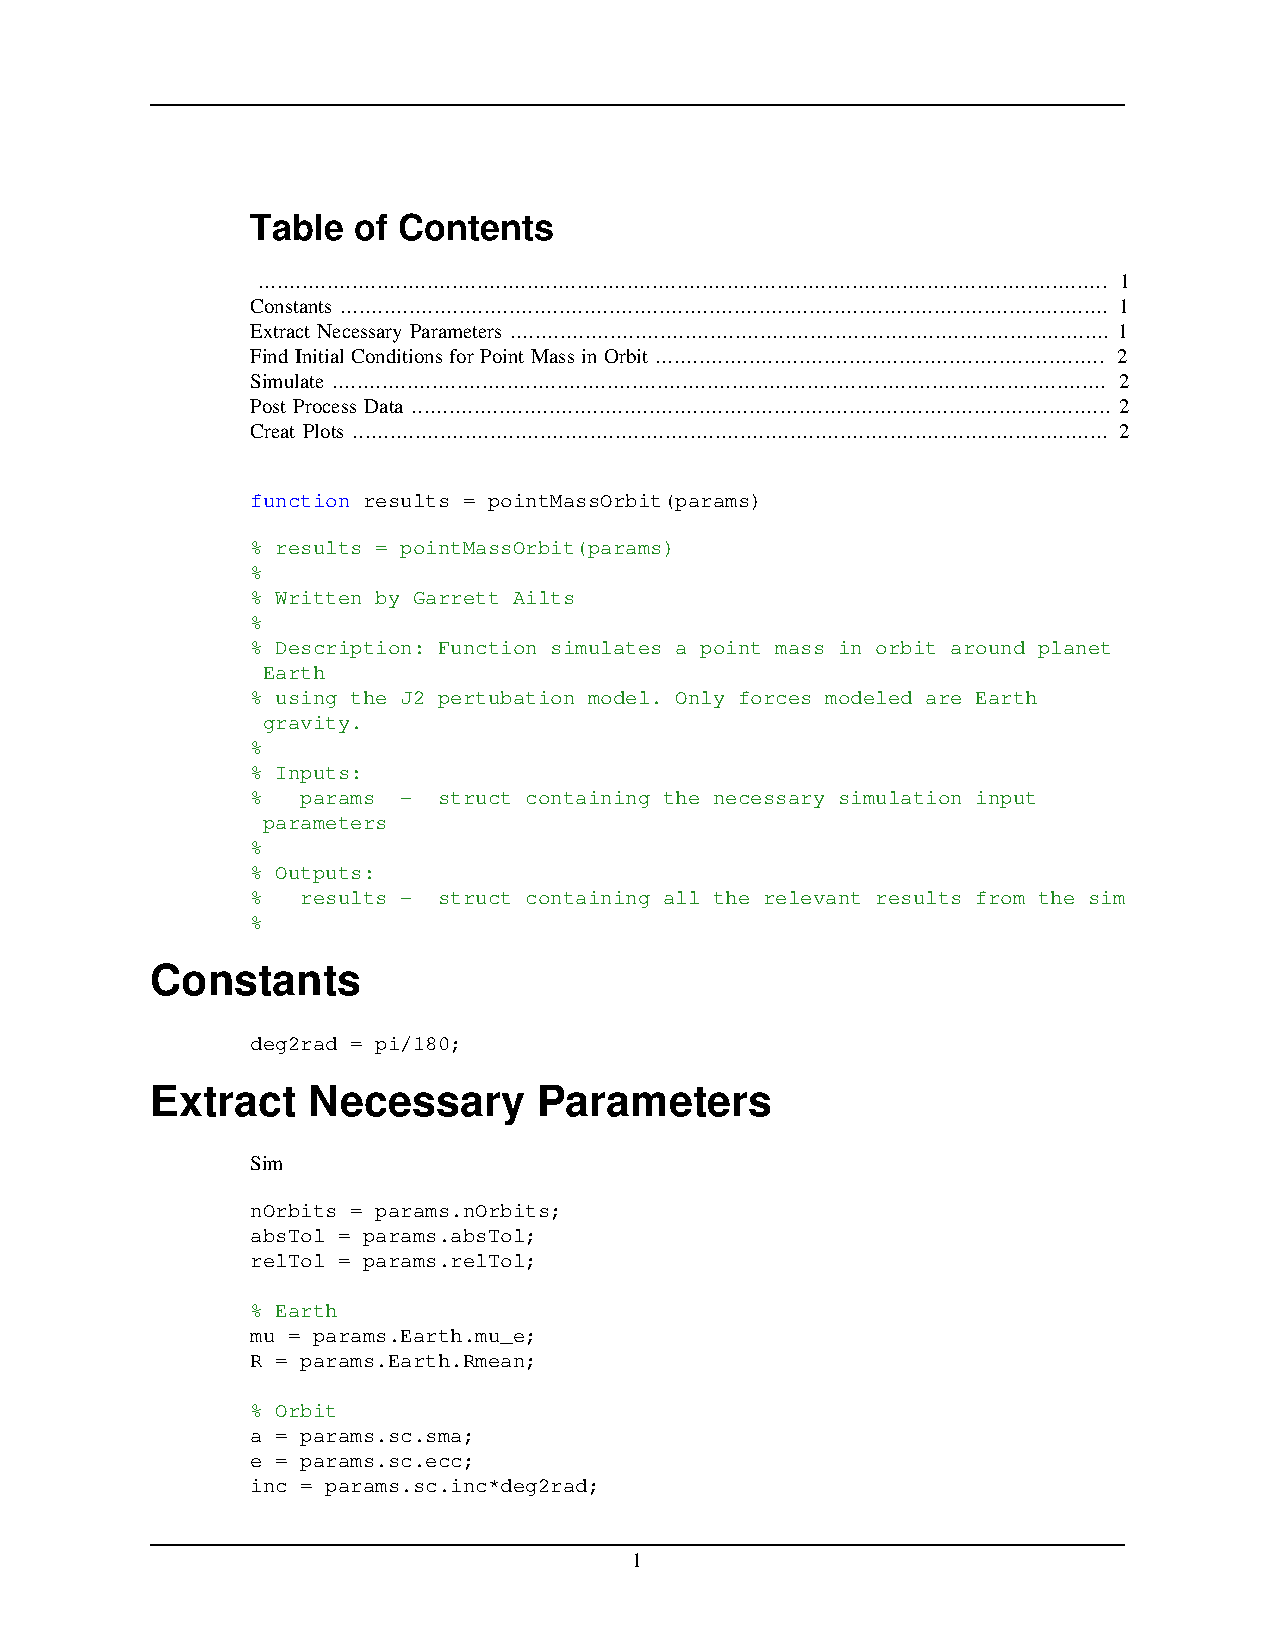
\includepdf[pages=-]{Semester_Project/docs/pdf/pointMassOrbit.pdf}
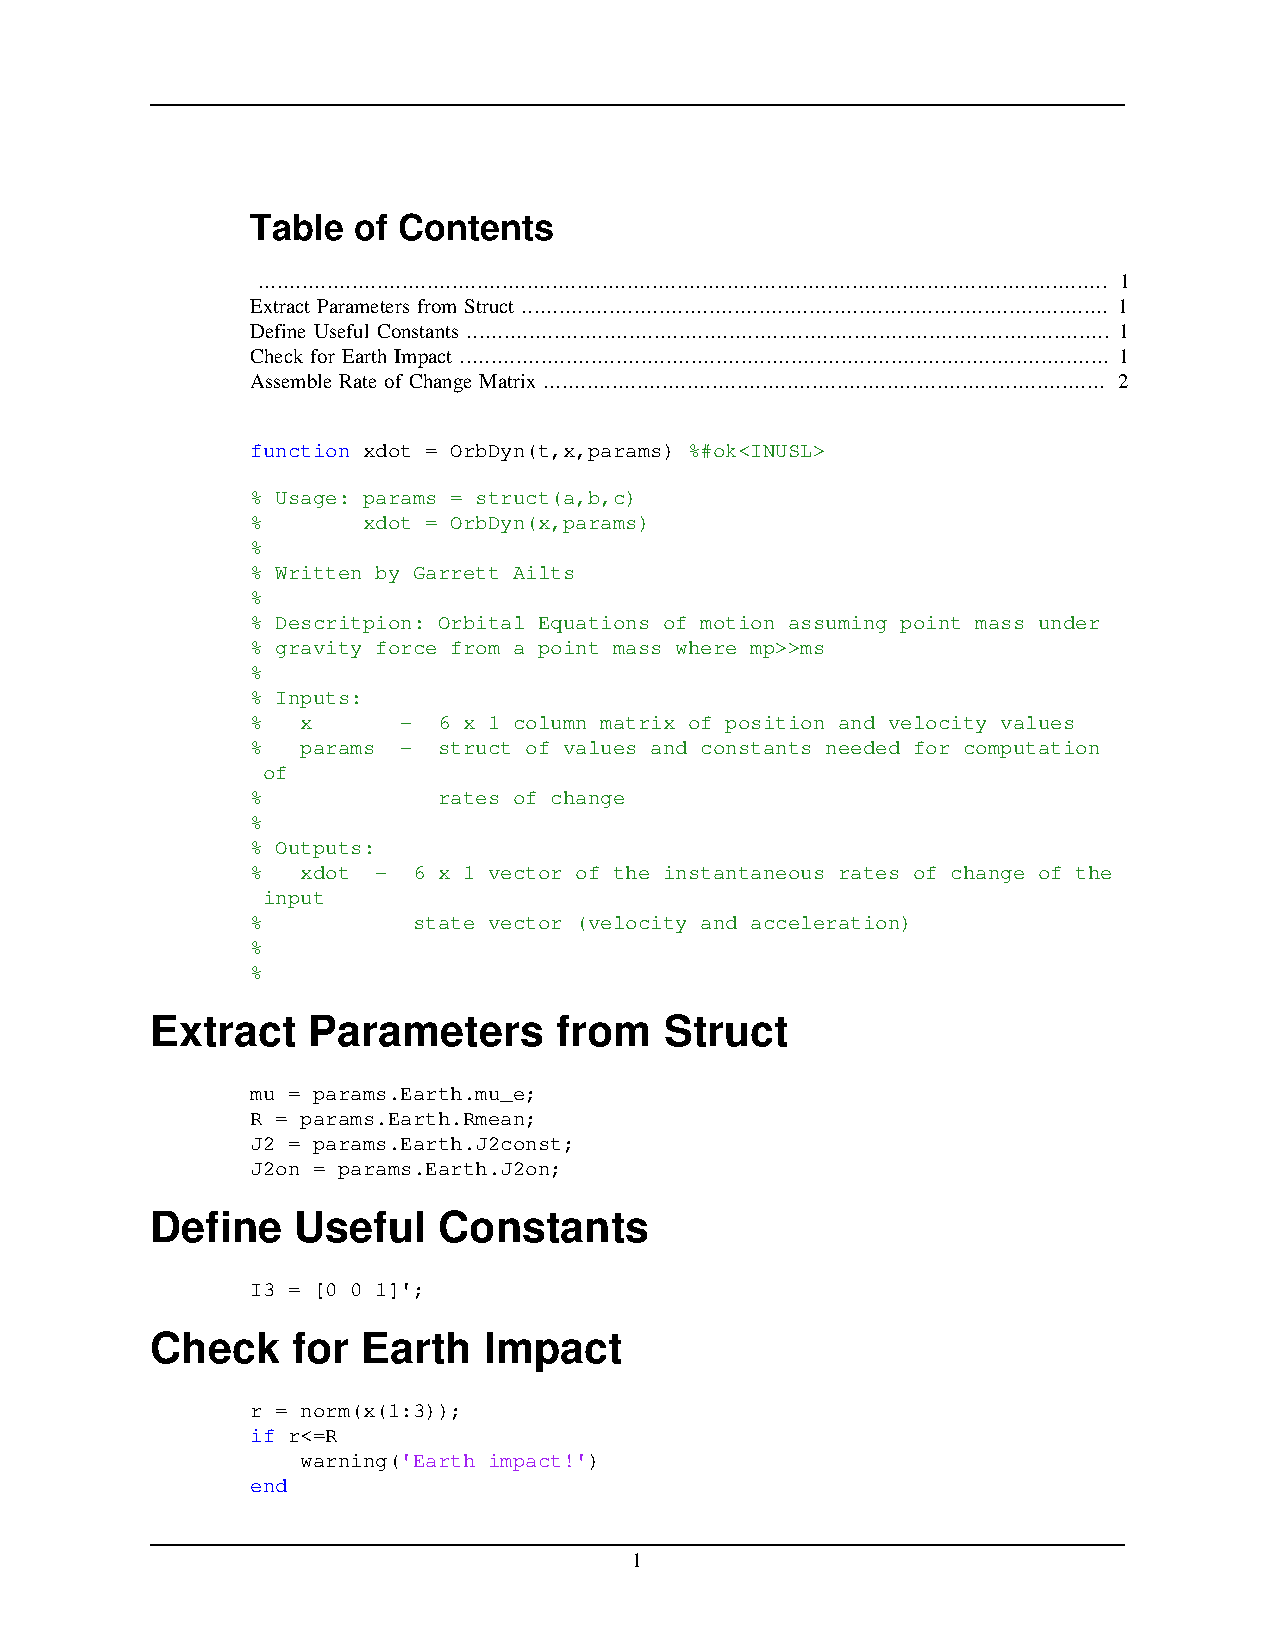
\includepdf[pages=-]{Semester_Project/docs/pdf/OrbDyn.pdf}
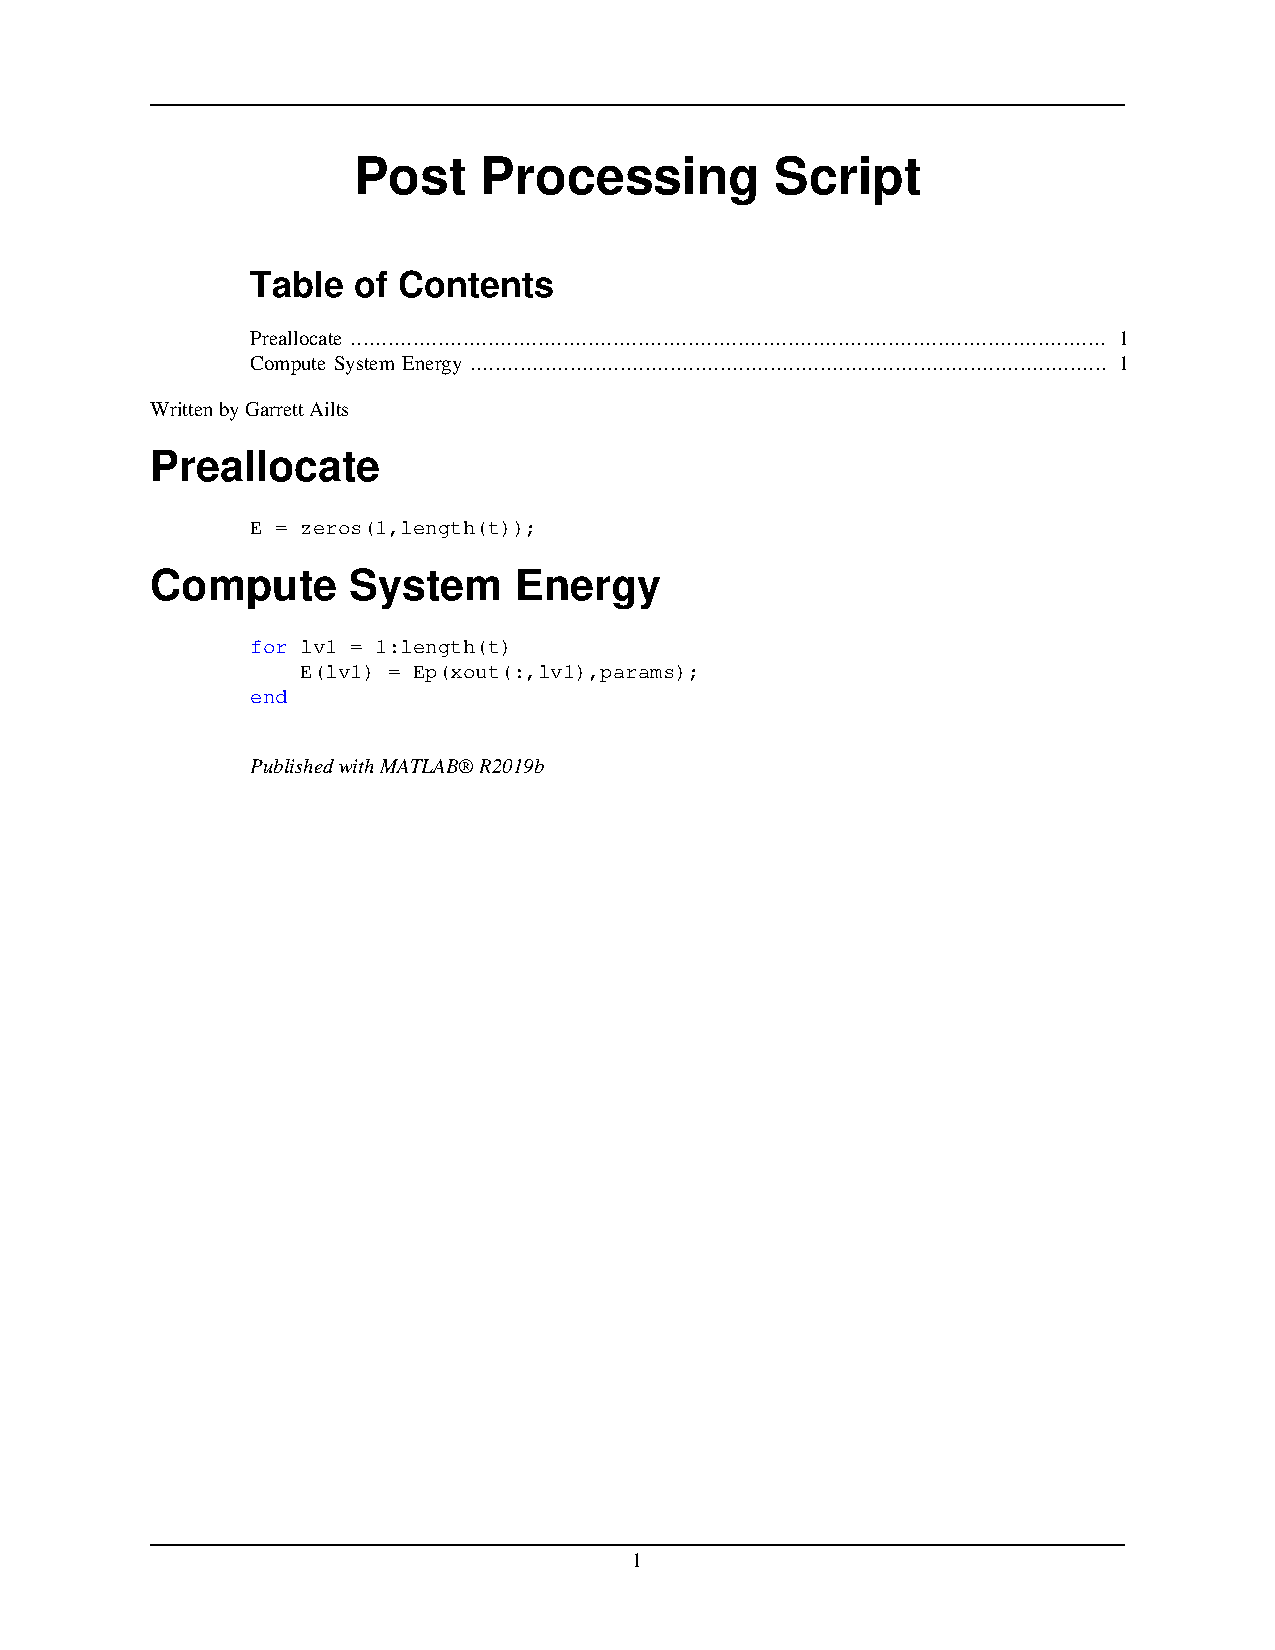
\includepdf[pages=-]{Semester_Project/docs/pdf/Post_Process}
 


%\VerbatimInput{Semester_Project/params/earthParams.txt}


\end{document}